\section{Exercice 3 - Détecteur de code - Fausse entrée négligée}

Il s'agit de répéter l'exercice 2 (section \ref{ex2}) mais en négligeant les fausses entrées.

\subsection{VHDL}

On propose la modélisation VHDL \textbf{comportementale} ci-dessous. Chaque fausse entrée est négligée. Il s'agit à nouveau de modéliser une \textbf{machine à états}.

\vhdl
\begin{lstlisting}
entity tp2_3 is
  port(PB_0,SW_0 : in bit;
       LED_0 : out bit);  
end tp2_3;

architecture Behavioral of tp2_3 is
begin
  process(PB_0)
  variable nbt : integer range 0 to 5;
  variable allume : bit := '0';
  begin
  if(PB_0'event and PB_0='1') then
    case nbt is
      when 0 =>
        if(SW_0='1') then
          nbt:=1;
        end if;
      when 1 =>
        if(SW_0='1') then
          nbt:=2;
        end if;
      when 2 =>
        if(SW_0='0') then
          nbt:=3;
        end if;
      when 3 =>
        if (SW_0 ='1') then
          nbt:=4;
        end if;
      when 4 =>
        nbt:=0;
        if(SW_0='0') then
          nbt:=5;
          allume := '1';
        end if;
      when 5 =>
        nbt:=0;
        allume:='0';
      end case;
      LED_0<=allume;
    end if;
  end process;        
end Behavioral;
\end{lstlisting}

Le code proposé ci-dessus permet d'ignorer les fausses entrées. Lorsqu'il y a une erreur elle n'est pas prise en compte et la machine à états reste inchangée.

\subsection{Synthèse}

\begin{figure}[!h]
   \centering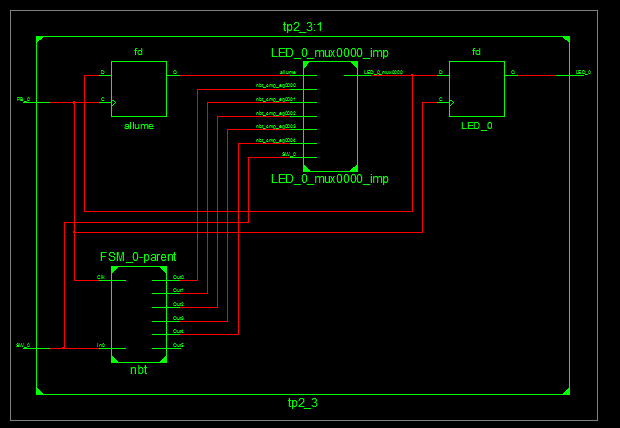
\includegraphics[width=0.74\textwidth]{files/tp2_3/rtl.png}
   \caption{Schéma RTL}
\end{figure}

\noindent Le nombre de bits d'état est étrangement le même que dans l'exercice 2.

\subsection{Différences par rapport à l'exercice 2}

On simule notre code à la même manière que dans l'exercice 2. On entre le bon code mais on glisse une erreur au milieu. Cette fois-ci l'erreur ne devrait pas être prise en compte et le code devrait être détecté :
\begin{figure}[!h]
   \centering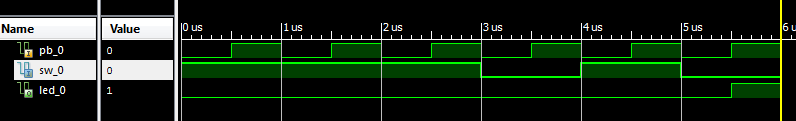
\includegraphics[width=\textwidth]{files/tp2_3/simu_erreur.png}
   \caption{Simulation}
\end{figure}

Notre simulation est concluante. Le troisième '1' était une erreur mais le code a tout de même été détecté. La fausse entrée a donc été négligée.